\documentclass[10pt]{article}

% %%%%%%%%%%%%%%%%%%%%%%%%%%%%%%%%%%%%%%%%%%%%%%%%%%%%%%%%%%%%%%%%%%%%%%%%%%%%%%
% %                                 PACKAGES                                   %
% %%%%%%%%%%%%%%%%%%%%%%%%%%%%%%%%%%%%%%%%%%%%%%%%%%%%%%%%%%%%%%%%%%%%%%%%%%%%%%
% Identifies input coming with an UTF-8 format
\usepackage[utf8]{inputenc}
% Uses 8-bit T1 fonts (Latin) 
\usepackage{setspace}
 \singlespacing
% Arial font.
\usepackage[scaled]{helvet}
\renewcommand\familydefault{\sfdefault}
\usepackage[T1]{fontenc}
\setlength{\parindent}{0.4cm}
% Equations
\usepackage{amsmath}
% Enum Item
\usepackage{enumitem}
% Easy Lists
\usepackage[ampersand]{easylist}
% Tables
\usepackage{booktabs}
\usepackage{longtable}
% Hyperreferences
\usepackage{hyperref}
% Images
\usepackage{graphicx}
% Set images location
\usepackage{wrapfig}
% Position for tables and images
\usepackage{float}
% Blibliography
\usepackage[backend=biber, style=numeric]{biblatex}
 \addbibresource{artAPA.bib}

% %%%%%%%%%%%%%%%%%%%%%%%%%%%%%%%%%%%%%%%%%%%%%%%%%%%%%%%%%%%%%%%%%%%%%%%%%%%%%%
% %                                  TITLE                                     %
% %%%%%%%%%%%%%%%%%%%%%%%%%%%%%%%%%%%%%%%%%%%%%%%%%%%%%%%%%%%%%%%%%%%%%%%%%%%%%%  
\title{
    Edge of Things: The Big Picture on the Integration of Edge, IoT and Cloud in
    a Distributed Computed Enviroment
}

\author{
Pablo Acereda\\
Computer Science Degree\\
}

% %%%%%%%%%%%%%%%%%%%%%%%%%%%%%%%%%%%%%%%%%%%%%%%%%%%%%%%%%%%%%%%%%%%%%%%%%%%%%%  
% %                                 DOCUMENT                                   %
% %%%%%%%%%%%%%%%%%%%%%%%%%%%%%%%%%%%%%%%%%%%%%%%%%%%%%%%%%%%%%%%%%%%%%%%%%%%%%%  
\begin{document}

% Creating title.
\maketitle

% %%%%%%%%%%%%%%%%%%%%%%%%%%%%%%%%% ABSTRACT %%%%%%%%%%%%%%%%%%%%%%%%%%%%%%%%%%%
\begin{abstract}

    As the usage of wireless networks and the Internet of Things (IoT) raise in
    popularity, that involves the risk of latency and traffic in the network.
    With the objective of the suppression of those obstacles the Edge Computing
    (EC) paradigm has been developed. With its integration the processing is
    carried in the edge of the network devices. EC is to increase the response
    time in the applications that previously used the cloud. The scope of this
    article is to prove the efficiency and resourcefulness of EC. As an
    addendum, the EC paradigm is compared with the rest of Cloud Computing
    Systems.

\end{abstract}

% %%%%%%%%%%%%%%%%%%%%%%%%%%%%%%%%% KEYWORDS %%%%%%%%%%%%%%%%%%%%%%%%%%%%%%%%%%%
{\bf Keywords:}
    IoT, 
    cloud computing, 
    edge computing, 
    fog computing, 
    multi-cloud.

\section{Introduction}

The Edge Computing (EC) new paradigm has incredible performing capabilities,
providing to most of the fields it is applied to a great improve in performance.
As mentioned in the article \cite{artiot}, the demmand for network and IoT
connected devices will increase at a great rate \cite{things} 
, as will its economic impact \cite{trillion} 
.

One of the advantages EC provides is the data processing before it is sent the
connection to the cloud takes place. That has a positive effect on the network
overhead, as well as in the security and privacy.

This new paradigm can be connected to many types of networks (MANETs, VANETs 
\hyperref[ecvanet]{\ref{ecvanet}} or ITSs).

\begin{figure}[h!]
 \centering
  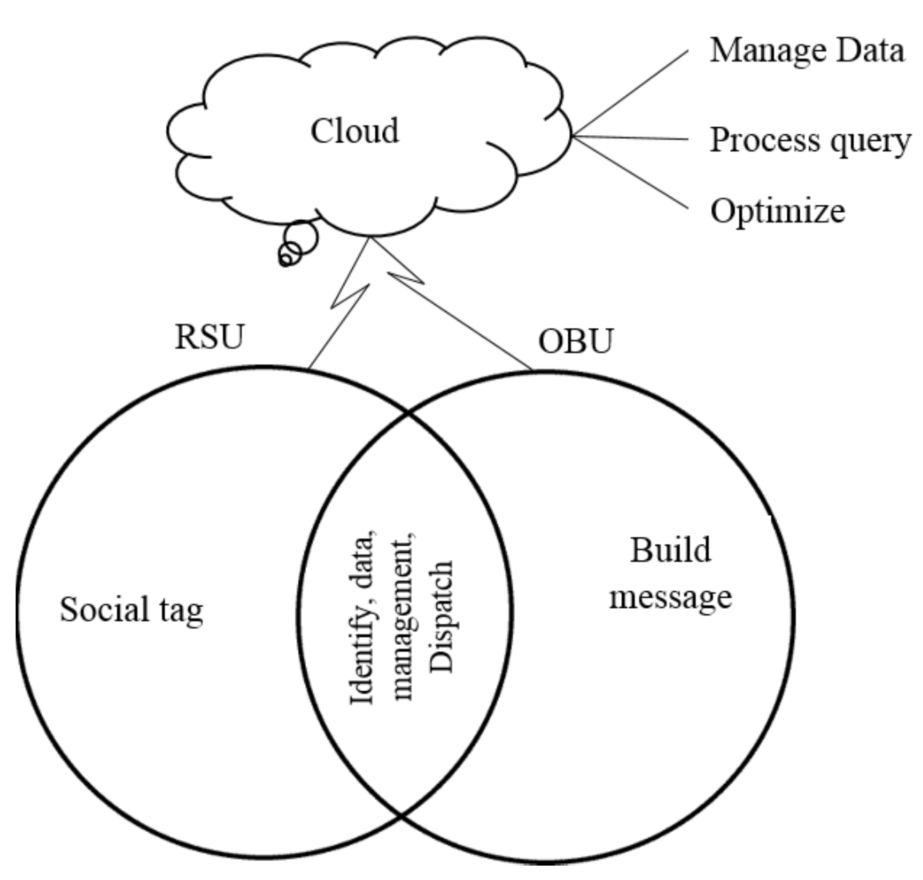
\includegraphics[width=0.6\textwidth]{ecVanet.png}
  \caption{EC in VANETs
   \label{ecvanet}}
\end{figure}

The original authors of the article \cite{artiot} claim that EC cannot
completely replace the cloud computing paradigm, as some applications still need
the support from the cloud or centrilized server. Furthermore, EC has problems
on its own, as there are part within its basis which need to be reconfigured or
redesigned.

\section{Overview of edge computing}

The demand on IoT services has been increasing for the past years and the Cloud
services cannot handle such a demand of that many users. It is therefore a
revolutionary idea to push the computing of the data to the edge of the network.

\subsection{Challenges Facing EC}

Some of the challenges faced when designing the EC architecture are introduced
in the following section \cite{artiot}. 

\begin{itemize}
    \item Device preferences must be chosen depending on the network
        requirements. Thus, to manage resources is a key point in the EC devices
        plan development.
    \item How devices fit within the network is a priority, not to overload
        their workload and drain their battery.
    \item In order not to waste the resources power, a schedule must be set to
        divide task among the edge (end-systems) and the cloud.
    \item The lack of a protocol to standarize communication among devices helps
        to reduce communication overhead (QoS).
    \item Connection shall be other key challenge in EC management. All the
        devices with high mobility experience desconnections or delayed
        communication.
    \item The edge of the network makes information more vulnerable to attacks.
        Therefore, the EC system shall implement a security system to handle
        such intrusions/attacks.
\end{itemize}

\begin{figure}[h!]
 \centering
  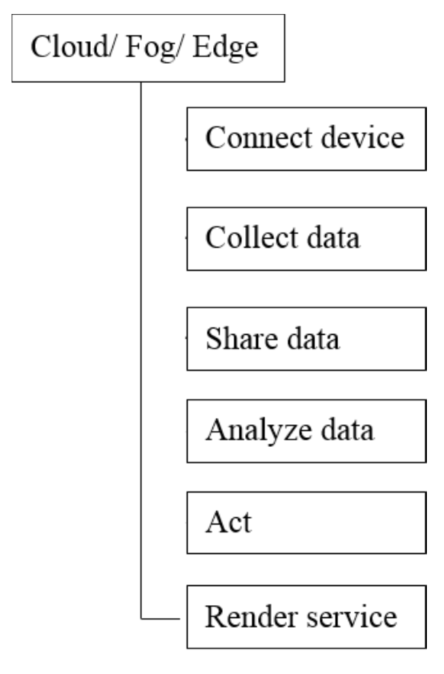
\includegraphics[width=0.4\textwidth]{ecTopography.png}
  \caption{EC topographues
   \label{ectopographies}}
\end{figure}

\section{An Overview of Computing Architecture}

Having EC provide a better quality-of-experience (QoE), the outcome of these
systems shall be compared to other architectures in order to prove its better
performance (comparison with fog computing (FC), cloud computing (CC) and
multi-cloud computing (MCC)). 

One of the aspects to take into account with EC is its multi-device
compatibility, as the end devices filter information (not sending to the
centralized server). Just as EC, FC pushed data treatment to the data source,
but in this case it is not the end device, but the Local Area Network (LAN). FC
is also used for IoT and real-time applications.

Other technology is the CC architecture, where the computations occurs in a
centralized server. The problem with this approach is the high latency and the 
heavy bandwidth usage between the server and the end devices (first and second 
layer respectively). As the server has to process huge quantities of data they
suffer from processing delay. In a similar way, MCC distributes servers.
Therefore, it has the same problems as CC, along with complexity and portability
issues. 

Compared to EC, the presented paradigm counts with greater scalability
and availability, as well as low latency and packet delay or jitter. On the 
other hand, as the computing power is pushed to the edge, the end devices set 
the bottleneck of the architecture. \cite{artiot}

\subsection{Research View on EC}

In academic and research backgrounds the EC algorithm has been used for its
numerous advantages, such as for example Augmente Reality (AR) processing 
\cite{arapps}. It has also been used for smart-cities applications \cite{mec} 
to prevent terrorist threats, natural calamities, etc \cite{artiot}.

After all these projects, a necessity came forward: the securitation of EC
urges. As the end nodes of the paradigm are directly the devices, where data is
treated firsthand, leads to potential insecurities.

\subsection{Service Benefits of EC}

The usage of the end nodes as edge servers brings a mitigation on the stress
bore by the network; increases performance for real time applications; also
reduces costs in the architecture, as the server does not need to be so
high-speced as in a, p.e., CC paradigm; among other advantages.

\subsection{Computing vs Storage Service of EC/FC/The Cloud/MCC}

The next section is better summarized in the following table
\hyperref[comparative]{\ref{comparative}}.

\begin{table}[h!]
 \begin{center}
  \begin{tabular}
      { | p{1.6cm} | p{2.3cm} | p{2.3cm} | p{2.3cm} | p{2.3cm} | }
  \hline
      & Edge Computing & Fog Computing & Cloud Computing & Multi Computing \\
  \hline
   \bf{Computing Service} 
      & Response time in milliseconds  
      & Response time in seconds to minutes based on the application 
      & Response time in minutes
      & Response time in minutes 
      \\
  \hline
   \bf{Storage Service}
      & Temporary storage, does not support huge data collections
      & Data can be stored for hours up to days
      & Permanent storage, supports huge data collections
      & Permanent storage, supports huge data collections and data protection
      \\
  \hline
  \end{tabular}
 \caption{Comparative analysis on computing services and storage services.
         \label{comparative}}
 \end{center}
\end{table}

\subsection{Computing in Heterogeneous Distributed Networks}

The past decade CC and MCC paradigms have been used as computing schemes, but
the exponential growth of the demands on the services produce an increase of the
network load, added to the already heavy traffic (due to the centralization of
servers), and the distance between end devices and server; new paradigms have
evolved for smart applications: EC or FC.

This paradigms allow to reduce data transfer (filterin and processing of data).
Thus, the avoidance of accidents and congestion in transportation is achieved.

\subsection{Privacy and Security Issues Relating to EC}

The architecture followed by EC also includes vulnerability problems, as the
data is treated at the edge of the network. EC needs a realiable system by which
edge server and end nodes can authenticate each other.

But, as data is so exposed, and specialiced (coming from end device), it also
shall be protected.

\section{Integration of IoT with Edges}

Nowaday, billions of IoT devices are constatly working (and expected to increase
in numbers), interconected, communicating, etc. To this devices, the CC
paradigms are quite obsolete, not being able to respond to those requests. With
this objective, EC is much more efficient as data transsion, processing and
storage is carried out by the end devices.

\section{Related Work}

The list of researches carried out with the use if IoT and EC is growing larger
by the day. For instance, Ali and Simeone developed a energy-efficient resource
allocation scheme for AR (Mobile EC); Amjad created a resour allocation
framework for IoT applications based on EC; Beraldi developed a cooperative load
balancing scheme (CooLoad) to reduce executation delay \cite{artiot}. And many 
other examples that do not need to even be mentioned in this article.

\section{Future Developments on EC}

IoT is extending, and it is being incorporated everywhere, threfore, a EC scheme
has to be able to process and communicate properly. Thus, it will need to
incorporate most of the specifications here discussed (offloading model; upgrade
in resource allocation; and effective scheduling algorithm).

\section{Conclusion}

It is true that Cloud Computing has experienced an increase in its current usage
over the past years, but saying its influence is over would be extremely foolish
of the reader. A more accurate representation of the future technological 
landscape would be one where Edge Computing starts being the most used paradigm 
for IoT application sees a considerable increase while Cloud Computing is still 
in use. Let's keep in mind, the fact that EC and FC have changed how data should
be treated for IoT, reducing the need of  powerful resources, it has experienced 
a deep rooting process since its inception. Explained in layman's terms, EC 
might be good, but CC isn't out of the game yet.


% Bibliography
\section*{Bibliography}
\printbibliography

\end{document}
